v\section{Case}
\textbf{Motivasjon og kriterie, romlig forventet standardavvik, fjerne usikkerhet i parametervalg} \\
\subsection{Case specification} 

\subsubsection{Input}
The only information that we're presented with beforehand is a variogram computed on the basis of some satelite data. This is however reckoned as slightly unreliable data and must be handled accordingly. The area in which the analysis will be based on is given as a list of xy-coordinates with each coordinate being given a z-variable denoting the numerical value to the attribute of interest. There is a total of 29116 coordinates, ordered into a rectangular grid with size 116 in x-direction and size 251 in y-direction. The directions will informally be called easting and northing when plotting. The variogram is presented in \ref{fig:variogram} along with the original data which we desire to predict. \\

\textbf{Modelspesifikasjon og utgangspunkt} \\
\subsubsection{Modelspecification and starting point of analysis} \label{subs:model}
As a necessary preliminary for the predictive analysis the height gradient attribute of all the coordinates is modelled as a stochastic variable. Attaining a Gaussian process to describe trend and variability of model one may view the grid as a GRF. The connection between variables in this model will revolve around spatial location within the grid, set in combination with stationarity we have that both the trendfunction and covariancefunction may be set to single-argument functions. \\
The model process may be fitted into the hierarchical model (HM) design described in \ref{model:hm}. With $Y$ denoting the temperature variables at locations $\vec{s}$, that's set to be distributed according to the Gaussian process, the process model follows as presented in %\ref{model:}
\begin{equation}
Y(\vec{s}) \sim \mathcal{MVN} \big( \ \mu(\vec{s}), \ \Sigma (\vec{s}) \big) 
\end{equation}
Here $\mu(\vec{s})$ denotes the trendfunction and $\Sigma((\vec{s})$ denotes the covariance function, both given easting-northing coordinates of the variables in question. \textbf{Noe mer her? Motivasjon for å velge Gaussisk fordeling} \\

With only a process model, one could have assumed noise-free sampling of data and started deriving results and predictions for the unobserved variables of the GRF. However, noise-free sampling may seem unreasonable in many settings. Gaussian distributed noise is a common way to model the unreliability of mearsurement equipment and/or random noise. Denoting the actual data being sampled from locations $\vec{s}$ in the GRF as $Z(\vec{s})$, the data model is then defined as:
\begin{equation}
Z(\vec{s}) \sim \mathcal{MVN} \big( \ Y(\vec{s}), \ \epsilon^2 I \big)
\end{equation}
Evidently, we assume that the noise is distributed independently on each sample with a single constant variance \textbf{Hvordan rimelig}. \\ 


\textbf{Utledning av framgangsmåte} \\
\subsection{Analysis}
\subsubsection{Theory}
With the data model and process model somewhat defined, the issue of choosing trend- and covariancefunctions arises. The discussion of covariancefunctions was covered in \ref{:covariance_functions}, and results will be presented for all three covariance functions shown in \ref{eq:covariance_functions}. \\ 

\subsubsection{Choosing prior-parameters}
As a consequence of defining our model with priordistributions for $\sigma^2$ and $\tau$, we must somehow estimate or choose parameters for their distributions. In order to do so, the variogram given as a part of the case preliminary has been utilized to estimate the GRF parameters of $\sigma^2$ and $\tau$. Given the three covariancefunctions in \ref{eq:covariance_functions}, the one may try to fit the the parameters of the chosen covariancefunction to the line. Denoting the discrete variogram values at points $k$ as $\gamma_k$ and the fitted covariancefunction at the same points as $\hat{\gamma}_k(\sigma^2, \tau)$, this is done by minimizing the associated lossfunction
\begin{equation}
Loss(\sigma^2, \tau) = \sum_k \bigg( \frac{\gamma_k - \hat{\gamma}_k(\sigma^2, \tau)}{\gamma_k} \bigg)^2
\end{equation}
Notice that we only have two parameters to be estimated for each covariancefunction as the nugget effect has been assumed to be negligible, resulting in more stable computation of fit. This minimization has been performed using the \textit{variofit} function in the \textit{geoR} package found in the programming environement R.vObviously, the covariance functions are exponentially decaying as a function of distance with the three chosen in \ref{eq:covariance_functions}. In order to visually compare the fit, we use the relation between the variogram of a stationary process and its covariancefunction that is
\begin{align} \label{eq:variogram_covariancefunction}
\begin{split}
    2\gamma(\textbf{s},\textbf{t}) &= Var(Y(\textbf{s}) - Y(\textbf{t})) \\
    &= Var(Y(\textbf{s})) + Var(Y(\textbf{t})) - 2Cov(Y(\textbf{s}),Y(\textbf{t})) \\
    \implies \gamma(\textbf{s},\textbf{t}) &= \sigma^2 - Cov(\|\textbf{s}-\textbf{t}\|) 
\end{split}
\end{align}

The variogram is then overlain with fitted covariancefunctions, adapted by equation \ref{eq:variogram_covariancefunction}, from \ref{eq:covariance_functions} in figure \ref{fiq:variogram_covariance}.  \\

Denoting the estimated values as $\hat{\sigma}^2$ and $\hat{\tau}$, one could have performed predictioning straight away. However, in an attempt to reduce the uncertainty in using this variogram, $\hat{\sigma}^2$ and $\hat{\tau}$ is used to fit parameters for the priors. This has been done by using a \textit{method of moments} inspired approach. As we have a single parameter prior for $\tau$, its mean and variance is estimated by 
\begin{align}
\hat{\lambda} = \frac{1}{\hat{\tau}}
\end{align}
With $\sigma^2$ given a gamma-prior, one needs to estimate two parameters. Denoting $\sum_k (\gamma_k - \hat{\sigma}^2)^2$ as $s_*^2$, the following approximation is used to set parameters $\alpha$ and $\beta$:
\begin{align}
\mathbf{E}(\sigma^2) = \frac{\alpha}{\beta} \approx \hat{\sigma}^2, \quad
\mathbf{Var}(\sigma^2) = \frac{\alpha}{\beta^2} \approx s_*^2 
\implies 
\hat{\alpha} = \frac{(\hat{\sigma}^2)^2}{s_*^2}, \quad  \hat{\beta} = \frac{\hat{\sigma}^2}{s_*^2}
\end{align}

The resulting prior-distributions are presented in figure \ref{fig:priors}.

\subsubsection{Discretizing the prior domains}
As the analysis relies on a numerical summation over the prior domains, a strategy must be defined to discretize the domains into $n_{\sigma^2}$ and $n_{\tau}$ divisions used the summation \ref{eq:expected_variance_grf_posterior}. In this case a method of \textit{stratified sampling} has been used. Given size-input $n_{\sigma^2}$, $(0,\inf)$ is subdivided into $n_{\sigma^2}$ divisions, each part corresponding to a $\frac{1}{n_{\sigma^2}}$ probability mass of the prior. Random samples are simulated until minimum one sample within each division is obtained. The same procedure is performed for $n_{\tau}$. 

The joined domain of $\tau$ and $\sigma^2$ is then considered a grid, with each cell corresponding to samples $(\tau_i, \sigma_j^2)$ having a probability mass of $\Delta_{ij} = \frac{1}{n_{\sigma^2} \cdot n_{\tau}}$ due to independence of priors. With both the normalizing constant and the summation for predictions using the same discretization, all $\Delta_{ij}$ cancels as they are independent of $(\tau_i, \sigma_j^2)$ and are therefore omitted from the calculations. A disadvantage is obviously the problem of simulating random samples for all the divisions if the number of divisions become high. However, $n_{\tau}$ and $n_{\sigma^2}$ is kept relatively low in this case. A visualization of the grid produced with the priors estimated from the variogram with $n_{\tau} = n_{\sigma^2} = 10$ is shown in figure \ref{fig:prior_grid}. 

\begin{figure}[!htb]
\hspace{-40pt}
   \begin{minipage}{0.475\textwidth}
     \centering
     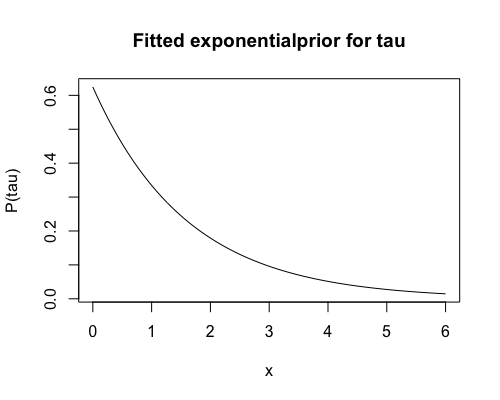
\includegraphics[width=1.3\linewidth]{figurer/fitted_exponential.png}
     \label{fig:data_original}
     \caption{Fitted prior distribution for $\tau$.}
   \end{minipage}\hfill
   \hspace{-40pt}
   \begin{minipage}{0.475\textwidth}
     \centering
     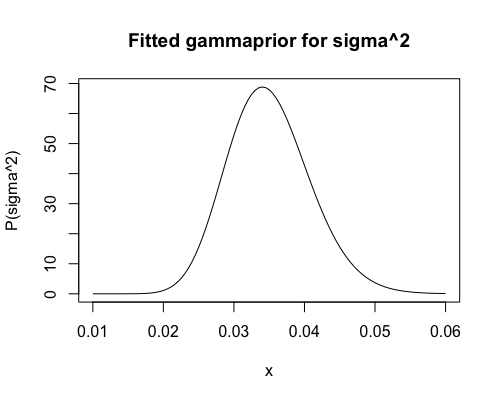
\includegraphics[width=1.3\linewidth]{figurer/fitted_gamma.png}
	 \label{fig:data_original_reduced}
	 \caption{Fitted prior distribution for $\sigma^2$}
	 \end{minipage}
\end{figure}
	
\begin{figure}[!htb]
\hspace{-50pt}
     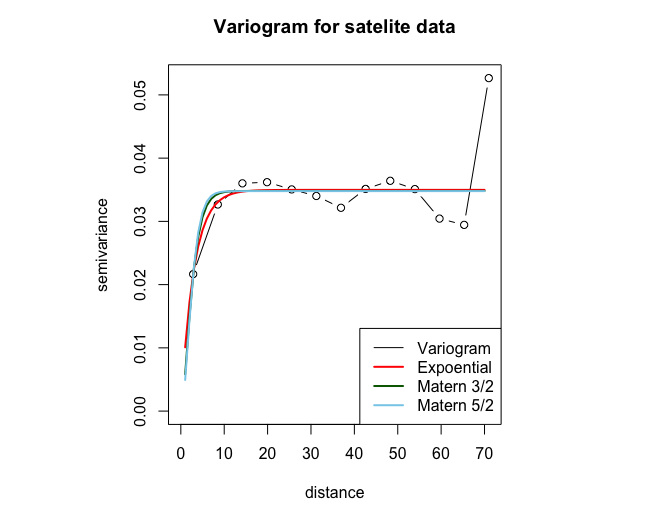
\includegraphics[width=1.3\linewidth]{figurer/variogram_covariancefunctions.png}
     \label{fig:variogram}
     \caption{Variogram with adapted correlationfunctions.}
\end{figure}



\textbf{Resultater} \\
